In this subsection we present our estimations for the different models based on data for the average household, and evaluate them. We find that the models with habit formation seem to perform best; they have better predictions and provide more sensible estimates. We conclude that our model with smoothed habit formation, estimated without an autocorrelation parameter, performs best.

We consider the following criteria most important for model selection:
\begin{enumerate}
    \item{} Model fit of the historic data.
    \item{} Ability to predict future consumption. This is important, as we will evaluate the impact of a carbon tax reform out-of-sample. 
    \item{} The intuition and interpretation of the estimated parameters of the models, especially how the models estimate the minimum consumption, and whether the size and sign of the estimated model parameters make sense.
\end{enumerate}
\\

The different criteria are evaluated by applying different measures and plots presented in the subsections below. We evaluate the model on data for the average household. The alternative, to evaluate the model for all income quintiles, would yield an unmanageable amount of information. Further, there is reason to believe that the data quality is highest for the average household, as it is an average of about 2,500 observation compared to around 500 for each quintile. 


Recall our estimation equation
\begin{align}
    w_{it} = \omega^i(z_t,\theta) = \frac{p_{it} b_{it}}{\mu_t} + \alpha_i \left( 1-\frac{\sum p_{kt}b_{kt}}{\mu_t}\right)+ u_{it}
\end{align}

We evaluate the following 8 models:
\begin{enumerate}[label={(\arabic*)}]
    \item Constant b: $b_{it} = b_i$ and $\rho=0$
    \item Constant b with autocorrelation parameter: $b_{it} = b_i$ $\rho \neq 0$
    \item Time trend: $b_{it} = b_i^* + \gamma t$ and $\rho=0$
    \item Time trend with autocorrelation parameter: $b_{it} = b_i^* + \gamma t$ and $\rho \neq 0$
    \item Habit formation: $b_{it} = b_i^* + \beta_i x_{i,t-1},$ and $\rho=0$
    \item Habit formation with autocorrelation parameter:$b_{it} = b_i^* + \beta_i x_{i,t-1},$ and $\rho \neq0$
    \item Smoothed habit formation: $ b_{it} = \beta_{1i} b_{i,t-1}  + \beta_{2i} x_{i,t-1}$ and $\rho=0$
    \item Smoothed habit formation with autocorrelation parameter: $ b_{it} = \beta_{1i} b_{i,t-1}  + \beta_{2i} x_{i,t-1}$ 
\end{enumerate}

\subsubsection{In-sample model fit}
To evaluate the in-sample model fit, we look at the log likelihood values and information criteria. We also assess the stability of the models with respect to starting values. We quantify this stability as the largest difference in estimated log likelihood values across different sets of starting values. 

We also calculate information criteria for the models. They are measures of the model fit taking into account the size of the model, since adding more parameters will per definition improve model fit and increase the log likelihood value. We employ Schwartz' Bayesian information criterion (BIC) as it includes a penalty for both the number of parameters and the number of observations \citep{lutkepohl2005new}, which is convenient when we have different numbers of observations for different models.
The Bayesian information criterion is calculated as
\begin{align}
    \text{BIC} = k \cdot ln (T) - 2  ln(\hat{L})
\end{align}
where $k$ is the number of parameters, $T$ is the number of observations and $ln(\hat{L})$ the log likelihood value.

\begin{table}[H]
\centering
\caption{Log Likelihood Value, BIC and stability}
\label{tableLV}
\begin{tabular}{lllllllll} \hline
Model         & (1)      & (2)      & (3)      & (4)      & (5)      & (6)      & (7)      & (8)      \\ \hline
BIC           & -1330 & -1433 & -1407 & -1429 & -1434 & -1423 & -1438 & -1382 \\
LV            & 735 & 788 & 787 & 799  & 799 & 795 & 802 & 773\\
LV difference & 0.098    & 0.350    & 6.163    & 5.167    & 12.525   & 4.023    & 17.105   & 8.632  \\ \hline
\end{tabular}
\captionsetup{singlelinecheck=off,size=scriptsize}
\setlength{\captionmargin}{10pt}
\caption*{
\textbf{Note:} Bla bla bla}
\end{table}
From table \ref{tableLV} it is obvious that model 1 and 2 - the simplest models - are more stable than models 3-8. This is partly expected, since model 1 and 2 only have one parameter in the minimum consumption specification - thus, the optimization problem is simpler, and the starting values only change for one parameter. If we look at models 5-8, which have almost the same number of parameters, we see that most stable models are model 6 and 8, that is the models in which we control for auto-correlation.

The Log Likelihood values (LV) are highest for model 7, 4 and 5. However the LV cannot directly be compared across models - here, the BIC is a more relevant metric, where the lowest value is preferred.  

Model 7 has by far the lowest BIC value, followed by model 5, 2, 4 and then 6. Models 1 and 8 have by far the highest BIC. Comparing the same models with and without auto-correlation, we see that model 2 and 4 performs better than model 1 and 3, indicating that it is important to include an auto-correlation parameter in those specifications. However, for the remaining models model 6 and 8 performs worse than model 5 and 7, indicating that when modeling habit formation as a function of past consumption, the model fit is not improved by controlling for auto-correlation. This finding is also present in the study by \cite{testing_les}, performing likelihood ratio tests of the specifications in \cite{pollak1969estimation}.

To examine the model fit, we plot the fitted values against the actual values of the budget share for each consumption group, see figure \ref{modelfit}. Based on these plots, we see that models 1, 2, 3 and 4 are generally not great at fitting the consumption shares. This is due to the assumptions of minimum consumption as either constant or linear in time being too restrictive. Models 6 and 8 does a decent job, while model 5 and 7 stands out as the best fits, as reflected by the BIC values.
\begin{figure}[H]
\centering
\caption{In sample fitted values}
\label{modelfit}
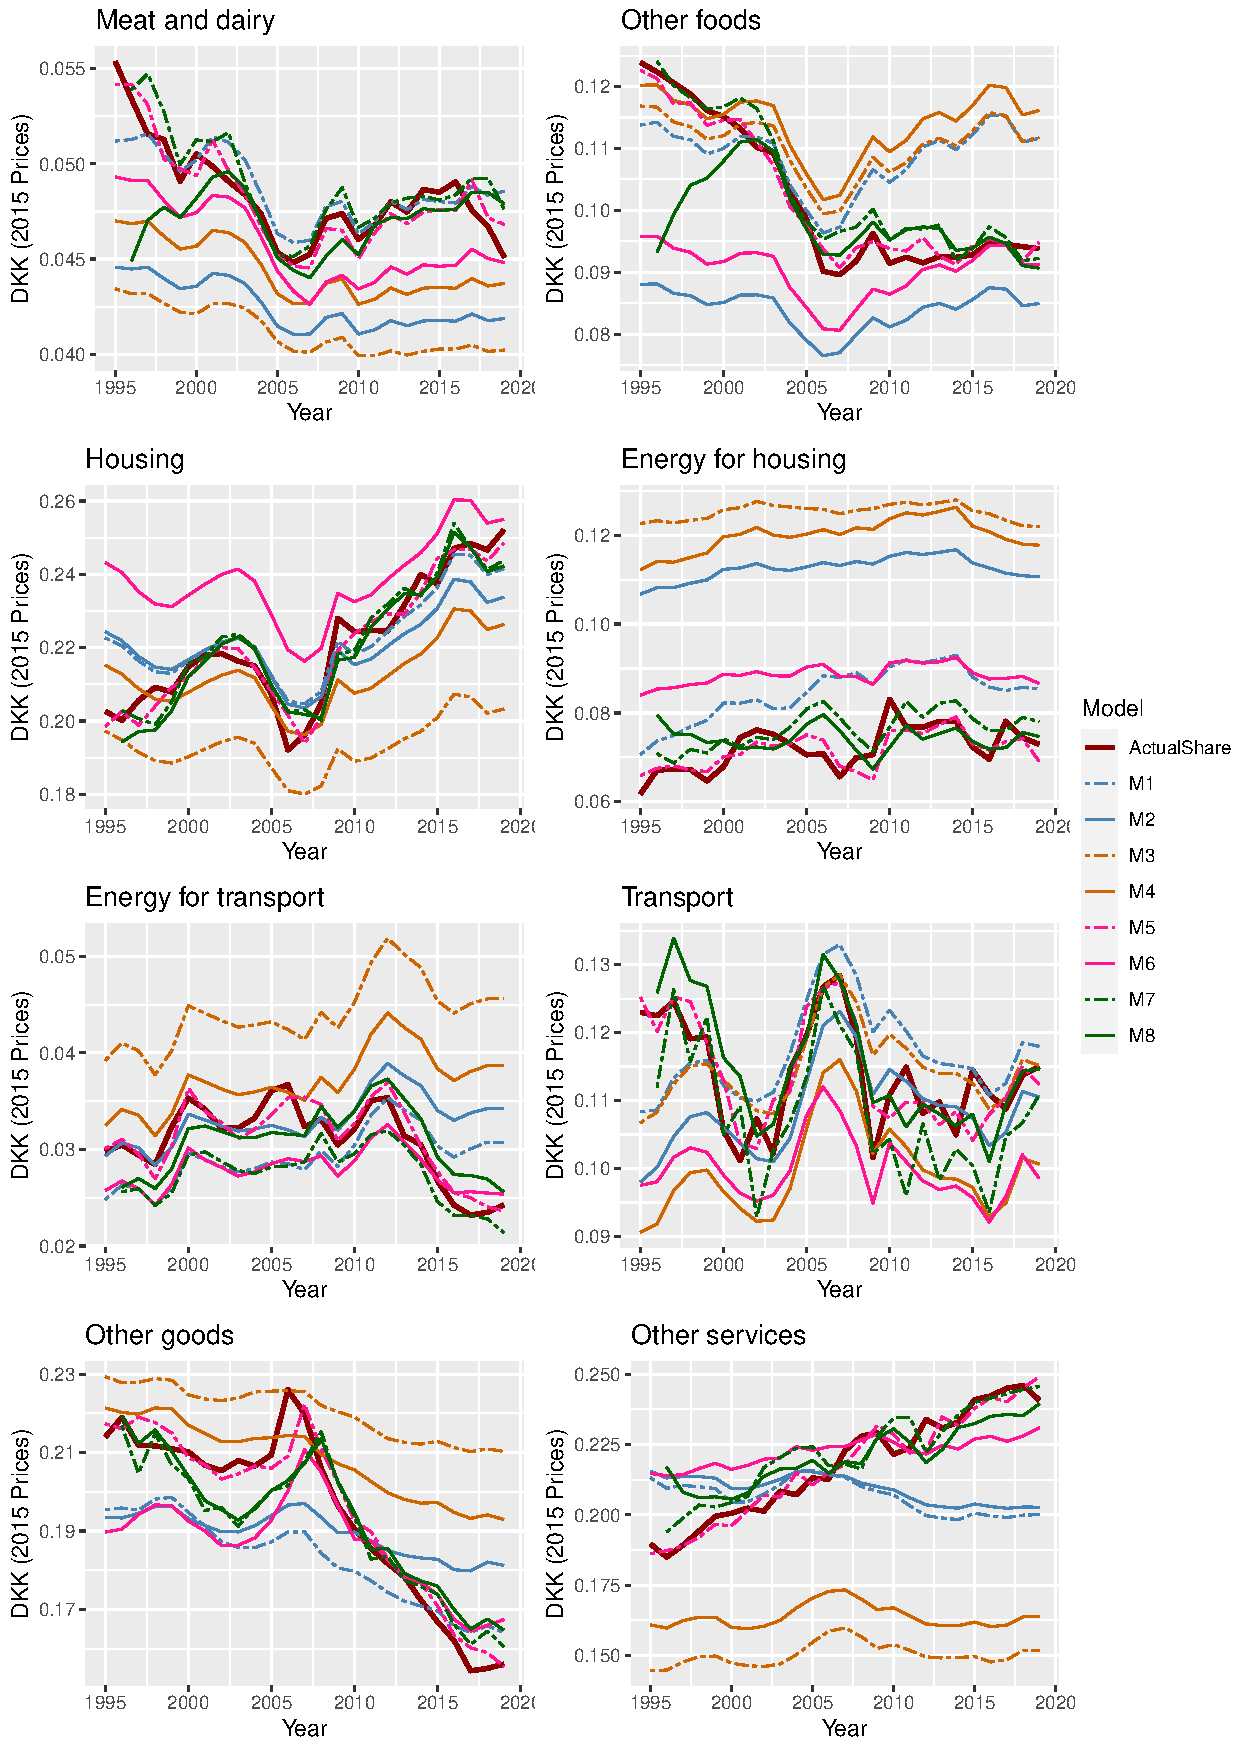
\includegraphics[width=.9\textwidth]{Figures/w_predict_heleperioden.pdf}
\captionsetup{singlelinecheck=off,size=scriptsize}
\setlength{\captionmargin}{10pt}
\caption*{
\textbf{Note:} bla bla bla bla bla}
\end{figure}

\subsubsection{Forecasting}

The out of sample fit is equally or even more important than the in sample fit, since we use the projection of consumption to address the distributional effects of a carbon tax. To get a measure for out of sample performance, we use the last years of the sample (year 2014-2019) as test data (that is the data used for evaluation). Using the last block of the sample for forecasting evaluation is the most common approach for non-stationary time-series data \citep{forecastingbergmeir}, since the time dependencies of the data are respected, and it corresponds to the later use of the system (the continuous forecasting of upcoming values).

We will use the last block of the sample to calculate two different measures. The first one is a simple forecast 6 years ahead, using the years 1994-2013 for estimation and the years 2014-2019 for forecasting. This approach is evaluated by simply plotting the forecasted budget shares for each model up against the actual budget shares, see figure \ref{forecast_fig}.

Acknowledging that the forecasting will be very dependent on the data leading up to the forecasting period, we apply time-series cross validation as a second measure of out of sample performance. The idea behind cross validation is to variate the data used for estimation (the training data) and the data used for forecasting (the test data). The cross validation approach makes the forecasting errors (here evaluated as the RMSE) less dependent on the chosen training and test data, as this is varied, and makes use of more information, since almost the whole data set is applied for training the model. The 8 models are thus trained by estimating on six training data sets that consists of the first 19 to 25 observations out of the 26 observations in the sample. The test set is for each training set just the next observation in the sample. 

This approach yields 6 prediction errors for each of the eight consumption groups for each of the eight models. We use the root mean squared error (RMSE) as accuracy measure, where K equals the number of predictions:
\begin{align}
    RMSE_i = \sqrt{\frac{\sum_k^K(\hat{w_{ik}}-w_{ik})^2}{K}}.
\end{align}

The forecasting is plotted in figure \ref{forecast_fig} together with the actual consumption shares. We see that model 2 and 6, which do not perform well in the in-sample fit, do a decent job predicting future consumption. Model 5 (which was probably the best in sample fit) is doing a poor job predicting future consumption. This indicates that model 5 is over-fitting to the existent data. Model 7 is doing a good job forecasting.
\begin{figure}[H]
\centering
\caption{Out of sample forecast (2014-2019)}
\label{forecast_fig}
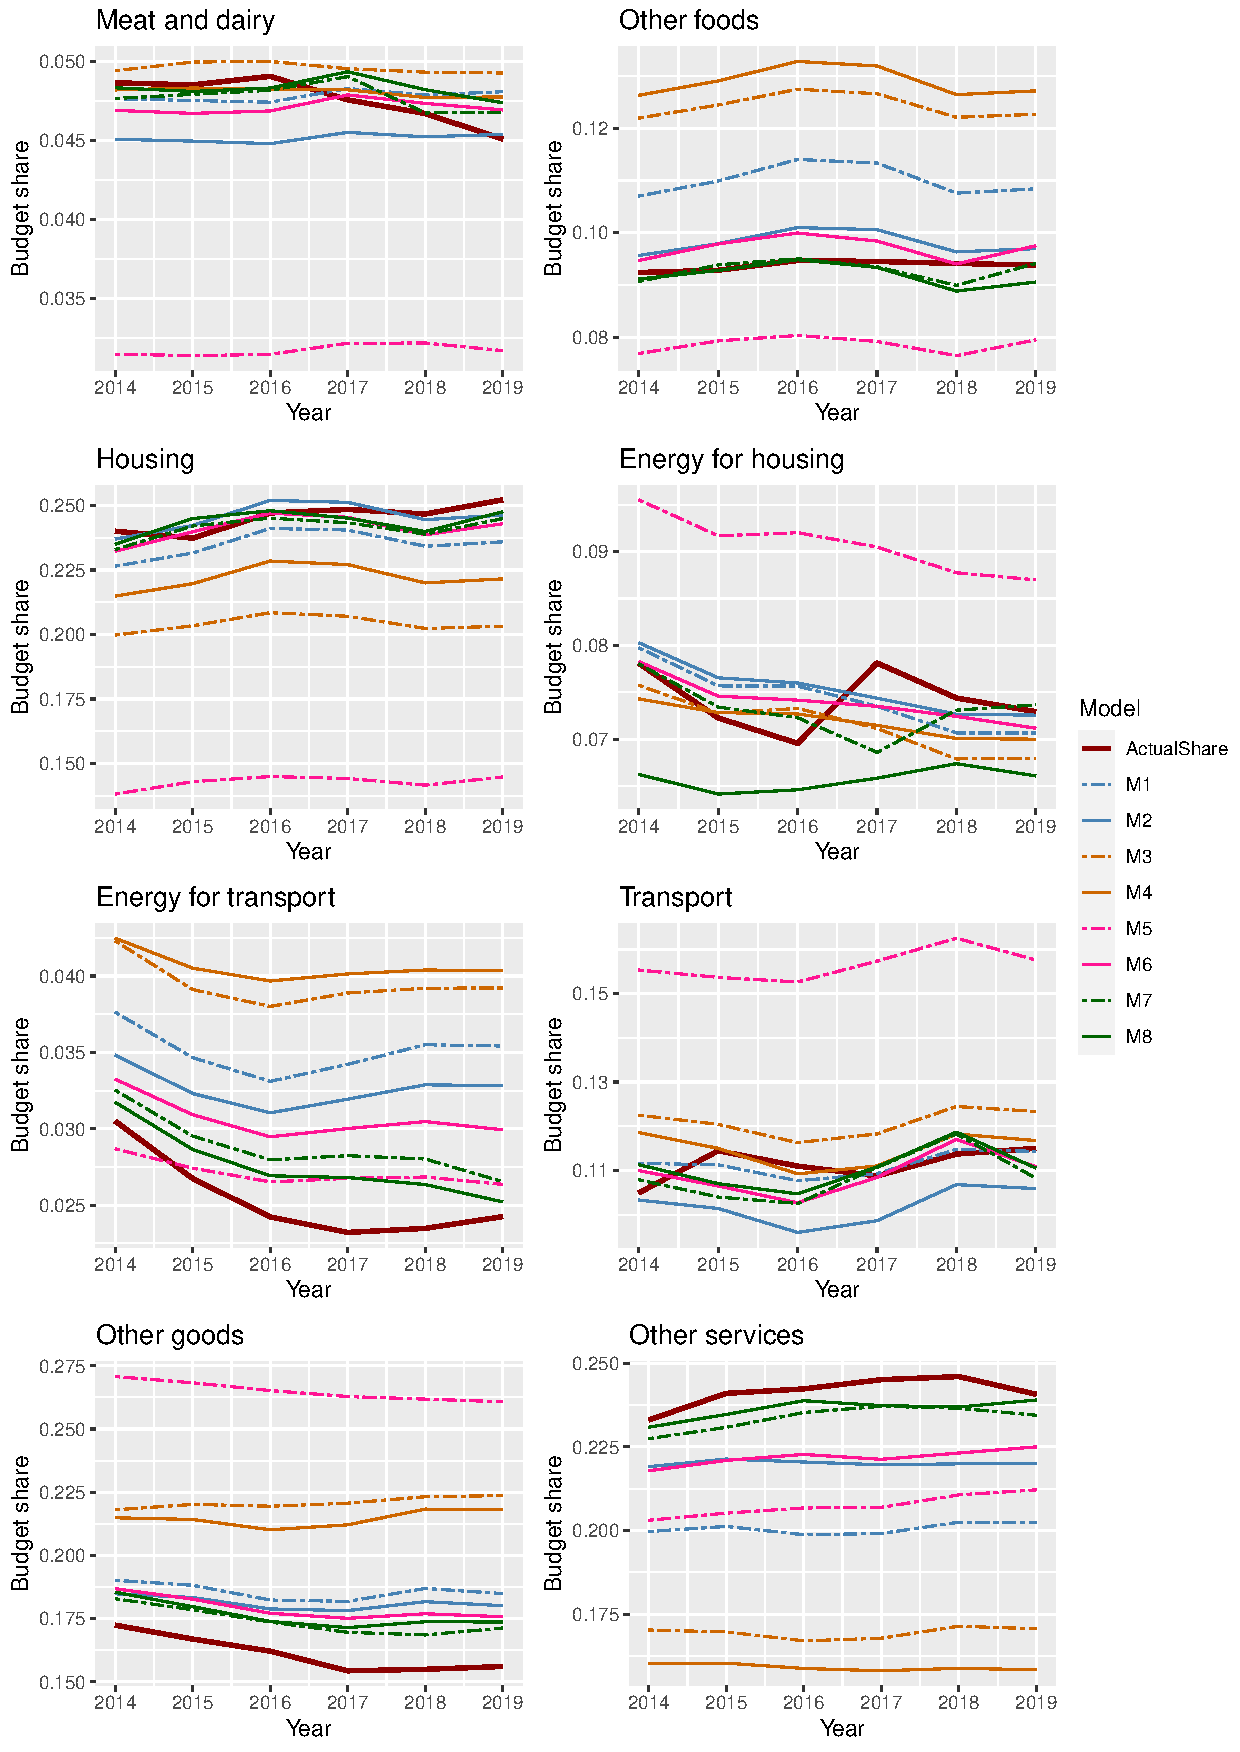
\includegraphics[width=.8\textwidth]{Figures/wforecast_ny.pdf}
\captionsetup{singlelinecheck=off,size=scriptsize}
\setlength{\captionmargin}{10pt}
\caption*{
\textbf{Note:} bla bla bla bla bla}
\end{figure}
\\
In table \ref{tableCV} below the different RMSE values for cross validation are presented as well as an average across consumption groups. We see that model 7 has the lowest RMSE when averaging over consumption groups, followed by model 6. Looking at the individual consumption groups, model 7 has the lowest error for almost all groups, only beaten by model 1 for Transport and model 6 for Housing. Overall model 2, 6 and 7 do a good job while model 1, 3, 4, 5 and 8 do a poorer job. This is somewhat the same conclusion we got from the 6 years ahead forecasting, however model 7 stands out as far the best out of sample predictor based on cross validation. 

\begin{table}[H]
\caption{RMSE based on cross validation}
\label{tableCV}
\begin{tabular}{@{}lllllllll@{}}
\hline
                  & (1) & (2) & (3)  & (4)& (5)  & (6) & (7) & (8) \\ \hline
Meat and dairy    & 0.0017   & 0.0027       & 0.0014 & 0.0114    & 0.0100 & 0.0020    & 0.0015       & 0.0146           \\
Other foods       & 0.0148   & 0.0036       & 0.0310 & 0.0314    & 0.0436 & 0.0039    & 0.0023       & 0.0057           \\
Housing           & 0.0092   & 0.0050       & 0.0322 & 0.0180    & 0.1422 & 0.0044    & 0.0065       & 0.0289           \\
Energy, housing   & 0.0039   & 0.0037       & 0.0051 & 0.0136    & 0.0275 & 0.0034    & 0.0027       & 0.0221           \\
Energy, transport & 0.0092   & 0.0063       & 0.0163 & 0.0203    & 0.0031 & 0.0049    & 0.0021       & 0.0153           \\
Transport         & 0.0034   & 0.0092       & 0.0089 & 0.0071    & 0.0766 & 0.0080    & 0.0066       & 0.0964           \\
Other goods       & 0.0219   & 0.0159       & 0.0631 & 0.0662    & 0.1089 & 0.0127    & 0.0094       & 0.0345           \\
Other services    & 0.0371   & 0.0135       & 0.0795 & 0.0951    & 0.0334 & 0.0143    & 0.0064       & 0.0869           \\ \hline
Average           & 0.0127   & 0.0075       & 0.0297 & 0.0329    & 0.0557 & 0.0067    & 0.0047       & 0.0381           \\ \hline 
\end{tabular}
\captionsetup{singlelinecheck=off,size=scriptsize}
\setlength{\captionmargin}{10pt}
\caption*{
\textbf{Note:} bla bla bla bla bla}
\end{table}

\subsubsection{Comparing the estimated minimum consumption levels}
Recall that demand for good $i$ in the linear expenditure system is given by
\begin{align}
    x_i &= b_i + \frac{\alpha_i}{p_i} \left ( \mu - \sum p_k b_k \right),
\end{align}
where the term $\mu - \sum p_k b_k $ is called the 'supernumerary income', or in plain words, the budget that is left after the minimum consumption needs have been fulfilled. A requirement for the LES is that the supernumerary income is greater than 0. Furthermore, $b_i$ should be lower than the observed consumption $x_i$, as the reverse would imply that minimum consumption needs are not met. For the LES to make intuitive sense, we need the $b$'s to be at least a bit lower than actual consumption. 

To evaluate the intution of the different estimates of minimum consumption, it is useful to plot how the minimum consumption levels (the $b$'s) evolve  throughout the sample period for each model and consumption group. These are shown in figure \ref{samlignb} in terms of actual consumption in 2015 prices instead of the budget shares. 

From these graphs, it is evident that model 1, 3, 4, and 5 are not providing realistic estimates of the minimum consumption. In the case of 1, 3 and 4, $b$ is estimated above actual consumption for several periods.  Model 5 is, for most goods, almost exactly estimated as lagged actual consumption, which we don't consider realistic either, and seems to be a case of over-fitting and over-stating of the habit coefficient. This is most likely the reason model 5 is performing well in sample but poorly out of sample. 

The rest of the models, 2, 6, 7, and 8, do provide realistic estimates of \textit{b} for most goods and periods. An example where this is not the case is model 6 of housing, where $b$ is estimated to be higher than actual consumption in the beginning of the period. Otherwise, the estimated b's look decent.
\begin{figure}[H]
\centering
\caption{Comparison of estimated b's for different models}
\label{samlignb}
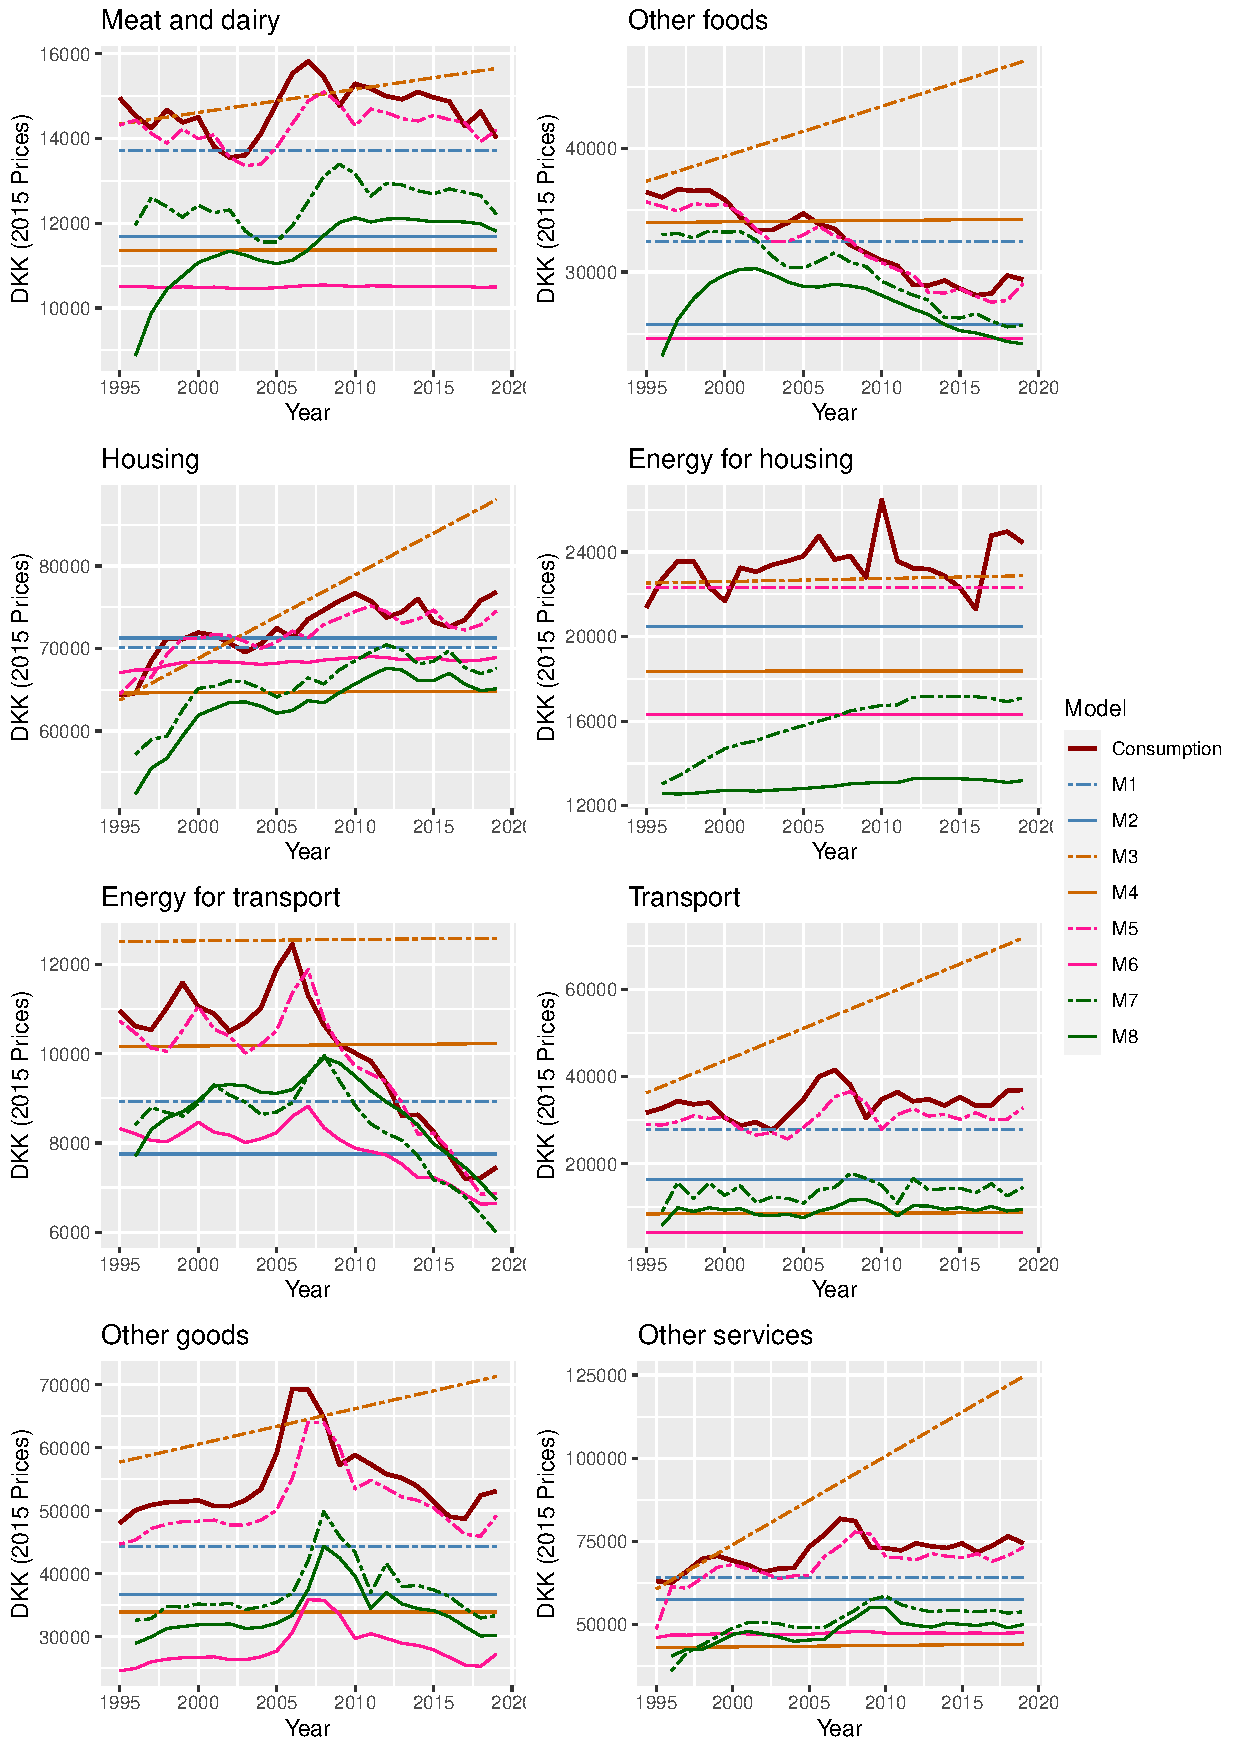
\includegraphics[width=.9\textwidth]{Figures/plot_min_ny.pdf}
\captionsetup{singlelinecheck=off,size=scriptsize}
\setlength{\captionmargin}{10pt}
\end{figure}

\subsubsection{Summary of model selection}
In table \ref{modelchoise} we attempt to summarize our different model evaluation findings. For each measure or plot each model gets a rating based on its performance.
\begin{table}[H]
\centering
\caption{Models rated in different criteria}
\label{modelchoise}
\resizebox{\textwidth}{!}{
\begin{tabular}{lcccccccc} \hline
Model         & (1) & (2)& (3)& (4)& (5)& (6) & (7)&(8) \\ \hline
Stability (starting values)  & Good & Good & Medium & Medium  & Bad & Medium & Bad & Medium\\
BIC           & Bad & Good & Medium & Good  & Good & Medium & Good & Bad\\
In-sample fit & Medium & Bad & Bad & Bad & Good & Medium & Good & Good \\
Estimated b's & Bad & Medium & Bad & Medium & Bad & Good  & Good & Medium  \\
Cross-validation & Medium & Good & Bad & Bad & Bad & Good & Good & Bad \\
Out of sample 6y & Medium & Good & Bad & Bad & Bad & Good & Good & Good  \\ \hline
\end{tabular} }
\end{table}
Overall, model 6 and 7 do best across the different criteria, followed by model 2. It stands out that model 7 does a good job across all criteria except the robustness to change in starting values. It is a challenge to choose good starting values for the AR process in (7) and (8), which might influence the stability of the model. As mentioned in section \ref{sec:habit_formation}, not controlling for autocorrelation can lead to overestimation of the coefficients in the habit equation. However, estimating habit formation partly as an AR(1) process might overcome this problem. Further, we evaluate small prediction errors more important for our analysis than finding unbiased coefficients. 

Bearing this in mind, we will continue our analysis using model 7, since it gives a nice intuitive measure of the habit formation in minimum consumption and a great in sample fit. Most importantly it is the best considered predictor of future consumption, which is highly relevant since the purpose of the model is to asses future consumption patterns. In the next section we present the estimation results.